\chapter{Introdução}
\lipsum[3-8]
%Olá Mundo!.
Hello World.

%Meu primeiro \textbf{texto} em \LaTeX.
My first draft using \LaTeX.

Já aprendi 10\% de \LaTeX.

A ativação de um neurônio é obtida por meio da equação $y_i = \frac{\sum_{i=0}^{N} x_i \times w_i }{\alpha}$.
Conforme Equação~\ref{eq:ativa}, a ativação de um neurônio é calculada...
A figura~\ref{fig:neuronio} ilustra um neurônio.

Mais detalhes serão apresentados na seção~\ref{sec:redes} e na Tabela~\ref{tab:notas}.

\begin{equation}
	y_i = \frac{\sum_{i=0}^{N} x_i \times w_i }{\alpha}
	\label{eq:ativa}
\end{equation}

\begin{figure}[htb]
	\centering
	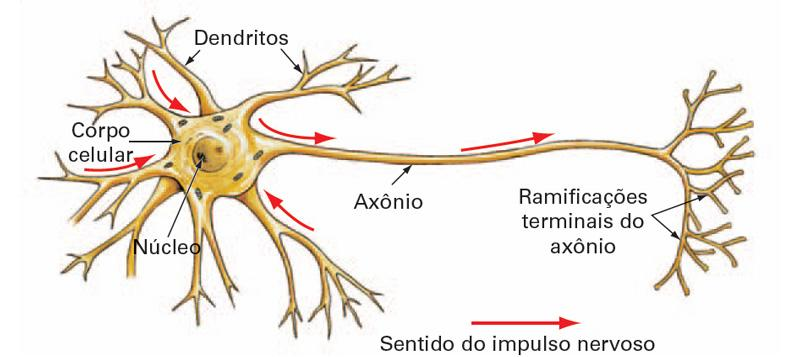
\includegraphics[scale=.4]{neuronio}
	\caption{Neurônio}\label{fig:neuronio}
\end{figure}

\begin{table}[htb]
	\caption{Notas}\label{tab:notas}
	\begin{tabular}{ccr}
		\hline
		\bf RA & \bf Nome & \bf Nota \\
		\hline
		12345 & Luciano & 7.0 \\
		56789 & Jose & 7.5 \\
		\hline
	\end{tabular}
\end{table}

\section{teste}